\chapter{Указатели}
\myindex{\CLanguageElements!\Pointers}
\label{label_pointers}

Указатели также часто используются для возврата значений из функции (вспомните случай со \scanf{}~(\myref{label_scanf})).

Например, когда функции нужно вернуть сразу два значения.

\section{Пример с глобальными переменными}

\lstinputlisting{patterns/061_pointers/global.c}

Это компилируется в:

\lstinputlisting[caption=\Optimizing MSVC 2010 (/Ob0)]{patterns/061_pointers/global.asm}

\myindex{\olly}
\clearpage
Посмотрим это в \olly:

\begin{figure}[H]
\centering
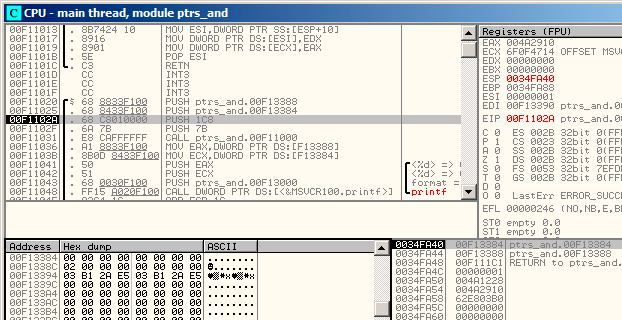
\includegraphics[scale=\FigScale]{patterns/061_pointers/olly_global1.png}
\caption{\olly: передаются адреса двух глобальных переменных в \ttfone}
\label{fig:pointers_olly_global_1}
\end{figure}

В начале адреса обоих глобальных переменных передаются в \ttfone.
Можно нажать \q{Follow in dump} на элементе стека и в окне слева 
увидим место в сегменте данных, выделенное для двух переменных.

Эти переменные обнулены, потому что по стандарту неинициализированные данные (\ac{BSS}) 
обнуляются перед началом исполнения: \cite[6.7.8p10]{C99TC3}.

\clearpage

И они находятся в сегменте данных, о чем можно удостовериться, нажав Alt-M и увидев карту памяти:

\begin{figure}[H]
\centering
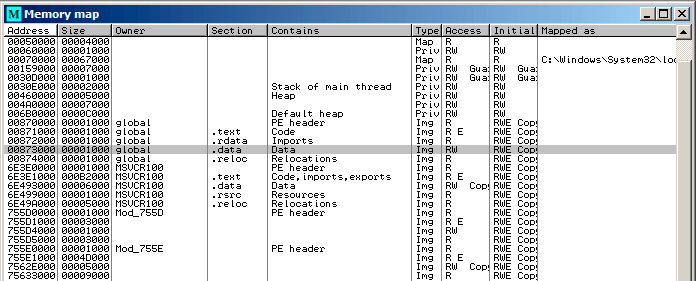
\includegraphics[scale=\FigScale]{patterns/061_pointers/olly_global5.png}
\caption{\olly: карта памяти}
\label{fig:pointers_olly_global_5}
\end{figure}

\clearpage
Трассируем (F7) до начала исполнения \ttfone: 

\begin{figure}[H]
\centering
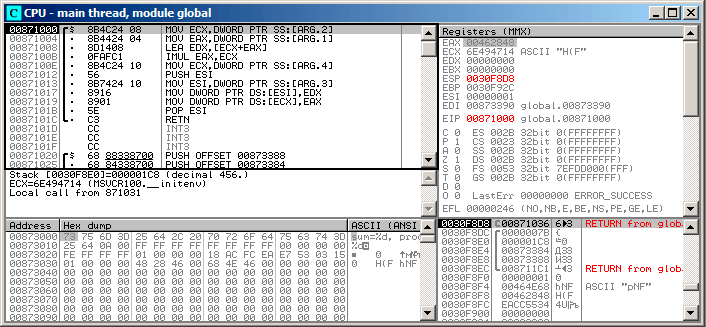
\includegraphics[scale=\FigScale]{patterns/061_pointers/olly_global2.png}
\caption{\olly: начало работы \ttfone}
\label{fig:pointers_olly_global_2}
\end{figure}

В стеке видны значения 456 (\TT{0x1C8}) и 123 (\TT{0x7B}), а также адреса двух глобальных переменных.

\clearpage
Трассируем до конца \ttfone.
Мы видим в окне слева, как результаты вычисления появились в глобальных переменных: 

\begin{figure}[H]
\centering
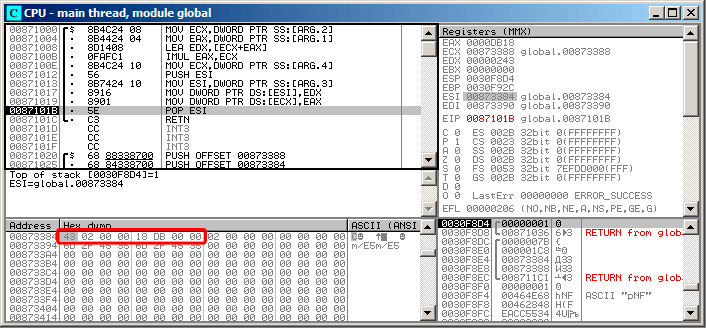
\includegraphics[scale=\FigScale]{patterns/061_pointers/olly_global3.png}
\caption{\olly: \ttfone заканчивает работу}
\label{fig:pointers_olly_global_3}
\end{figure}

\clearpage
Теперь из глобальных переменных значения загружаются в регистры для передачи в \printf :

\begin{figure}[H]
\centering
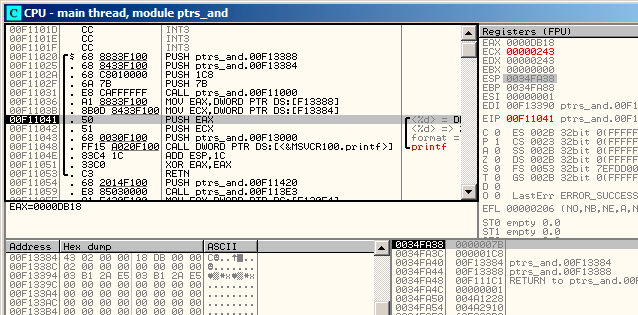
\includegraphics[scale=\FigScale]{patterns/061_pointers/olly_global4.png}
\caption{\olly: адреса глобальных переменных передаются в \printf}
\label{fig:pointers_olly_global_4}
\end{figure}

\section{Пример с локальными переменными}

Немного переделаем пример:

\lstinputlisting[caption=теперь переменные локальные]{patterns/061_pointers/local_RU.c}

Код функции \ttfone не изменится.
Изменится только \main:

\lstinputlisting[caption=\Optimizing MSVC 2010 (/Ob0)]{patterns/061_pointers/local.asm}

\newcommand{\PtrsAddresses}{\TT{0x2EF854} и \TT{0x2EF858}\xspace}

\clearpage
Снова посмотрим в \olly.
Адреса локальных переменных в стеке это \PtrsAddresses.
Видно, как они заталкиваются в стек: 

\begin{figure}[H]
\centering
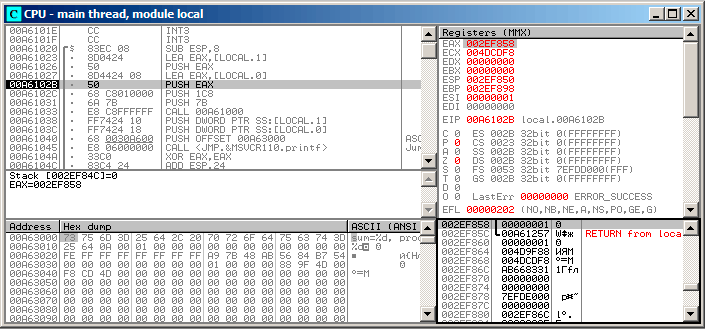
\includegraphics[scale=\FigScale]{patterns/061_pointers/olly_stk1.png}
\caption{\olly: адреса локальных переменных заталкиваются в стек}
\label{fig:pointers_olly_stk_1}
\end{figure}

\clearpage
Начало работы \ttfone.
В стеке по адресам \PtrsAddresses пока находится случайный мусор:

\begin{figure}[H]
\centering
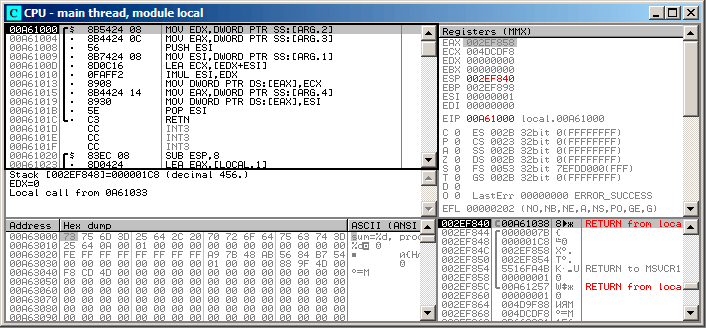
\includegraphics[scale=\FigScale]{patterns/061_pointers/olly_stk2.png}
\caption{\olly: \ttfone начинает работу}
\label{fig:pointers_olly_stk_2}
\end{figure}

\clearpage
Конец работы \ttfone:

\begin{figure}[H]
\centering
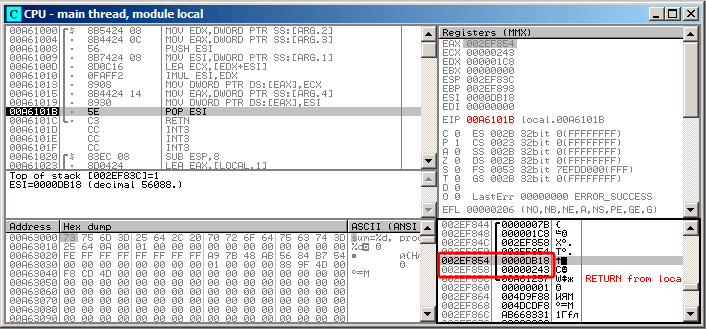
\includegraphics[scale=\FigScale]{patterns/061_pointers/olly_stk3.png}
\caption{\olly: \ttfone заканчивает работу}
\label{fig:pointers_olly_stk_3}
\end{figure}

В стеке по адресам \PtrsAddresses теперь находятся значения \TT{0xDB18} и \TT{0x243}, это результаты работы \ttfone.

\section{\Conclusion{}}

\ttfone может одинаково хорошо возвращать результаты работы в любые места памяти. 
В этом суть и удобство указателей.
Кстати, \IT{references} в \Cpp работают точно так же. Читайте больше об этом: (\myref{cpp_references}).

